\documentclass[twoside]{book}

% Packages required by doxygen
\usepackage{fixltx2e}
\usepackage{calc}
\usepackage{doxygen}
\usepackage[export]{adjustbox} % also loads graphicx
\usepackage{graphicx}
\usepackage[utf8]{inputenc}
\usepackage{makeidx}
\usepackage{multicol}
\usepackage{multirow}
\PassOptionsToPackage{warn}{textcomp}
\usepackage{textcomp}
\usepackage[nointegrals]{wasysym}
\usepackage[table]{xcolor}

% Font selection
\usepackage[T1]{fontenc}
\usepackage[scaled=.90]{helvet}
\usepackage{courier}
\usepackage{amssymb}
\usepackage{sectsty}
\renewcommand{\familydefault}{\sfdefault}
\allsectionsfont{%
  \fontseries{bc}\selectfont%
  \color{darkgray}%
}
\renewcommand{\DoxyLabelFont}{%
  \fontseries{bc}\selectfont%
  \color{darkgray}%
}
\newcommand{\+}{\discretionary{\mbox{\scriptsize$\hookleftarrow$}}{}{}}

% Page & text layout
\usepackage{geometry}
\geometry{%
  a4paper,%
  top=2.5cm,%
  bottom=2.5cm,%
  left=2.5cm,%
  right=2.5cm%
}
\tolerance=750
\hfuzz=15pt
\hbadness=750
\setlength{\emergencystretch}{15pt}
\setlength{\parindent}{0cm}
\setlength{\parskip}{3ex plus 2ex minus 2ex}
\makeatletter
\renewcommand{\paragraph}{%
  \@startsection{paragraph}{4}{0ex}{-1.0ex}{1.0ex}{%
    \normalfont\normalsize\bfseries\SS@parafont%
  }%
}
\renewcommand{\subparagraph}{%
  \@startsection{subparagraph}{5}{0ex}{-1.0ex}{1.0ex}{%
    \normalfont\normalsize\bfseries\SS@subparafont%
  }%
}
\makeatother

% Headers & footers
\usepackage{fancyhdr}
\pagestyle{fancyplain}
\fancyhead[LE]{\fancyplain{}{\bfseries\thepage}}
\fancyhead[CE]{\fancyplain{}{}}
\fancyhead[RE]{\fancyplain{}{\bfseries\leftmark}}
\fancyhead[LO]{\fancyplain{}{\bfseries\rightmark}}
\fancyhead[CO]{\fancyplain{}{}}
\fancyhead[RO]{\fancyplain{}{\bfseries\thepage}}
\fancyfoot[LE]{\fancyplain{}{}}
\fancyfoot[CE]{\fancyplain{}{}}
\fancyfoot[RE]{\fancyplain{}{\bfseries\scriptsize Generated by Doxygen }}
\fancyfoot[LO]{\fancyplain{}{\bfseries\scriptsize Generated by Doxygen }}
\fancyfoot[CO]{\fancyplain{}{}}
\fancyfoot[RO]{\fancyplain{}{}}
\renewcommand{\footrulewidth}{0.4pt}
\renewcommand{\chaptermark}[1]{%
  \markboth{#1}{}%
}
\renewcommand{\sectionmark}[1]{%
  \markright{\thesection\ #1}%
}

% Indices & bibliography
\usepackage{natbib}
\usepackage[titles]{tocloft}
\setcounter{tocdepth}{3}
\setcounter{secnumdepth}{5}
\makeindex

% Hyperlinks (required, but should be loaded last)
\usepackage{ifpdf}
\ifpdf
  \usepackage[pdftex,pagebackref=true]{hyperref}
\else
  \usepackage[ps2pdf,pagebackref=true]{hyperref}
\fi
\hypersetup{%
  colorlinks=true,%
  linkcolor=blue,%
  citecolor=blue,%
  unicode%
}

% Custom commands
\newcommand{\clearemptydoublepage}{%
  \newpage{\pagestyle{empty}\cleardoublepage}%
}

\usepackage{caption}
\captionsetup{labelsep=space,justification=centering,font={bf},singlelinecheck=off,skip=4pt,position=top}

%===== C O N T E N T S =====

\begin{document}

% Titlepage & ToC
\hypersetup{pageanchor=false,
             bookmarksnumbered=true,
             pdfencoding=unicode
            }
\pagenumbering{alph}
\begin{titlepage}
\vspace*{7cm}
\begin{center}%
{\Large ssbm-\/py }\\
\vspace*{1cm}
{\large Generated by Doxygen 1.8.13}\\
\end{center}
\end{titlepage}
\clearemptydoublepage
\pagenumbering{roman}
\tableofcontents
\clearemptydoublepage
\pagenumbering{arabic}
\hypersetup{pageanchor=true}

%--- Begin generated contents ---
\chapter{R\+E\+A\+D\+ME}
\label{md__r_e_a_d_m_e}
\Hypertarget{md__r_e_a_d_m_e}
This is an in-\/progress project designed to be a utility for S\+S\+BM Streamers using O\+BS

Project Goals\+:
\begin{DoxyItemize}
\item Create a comprehensive but simple class for an S\+S\+BM Match
\item Develop a G\+UI with a system to store, record, and manipulate Match data
\item Use challonge.\+com\textquotesingle{}s A\+PI to link challonge matches to Match objects
\item Provide a suite of misc. tools to interact with O\+BS though plugins/files
\end{DoxyItemize}

Development is ongoing and likely unstable until further notice. This repo is primarily for my personal use and organization

TO DO\+:
\begin{DoxyItemize}
\item Create Match class
\item Create T\+Kinter G\+UI
\item Link T\+Kinter G\+UI with the Match class
\item Write file manipulation functions
\item Integrate Challonge
\item Document with Doxygen
\item Get a stable version
\item Test/debug on different systems 
\end{DoxyItemize}
\chapter{Todo List}
\label{todo}
\Hypertarget{todo}

\begin{DoxyRefList}
\item[\label{todo__todo000001}%
\Hypertarget{todo__todo000001}%
File \hyperlink{gui_8py}{gui.py} ]testing this
\begin{DoxyItemize}
\item This is one item
\item This is another item
\item Testing this thing 
\end{DoxyItemize}
\end{DoxyRefList}
\chapter{Hierarchical Index}
\section{Class Hierarchy}
This inheritance list is sorted roughly, but not completely, alphabetically\+:\begin{DoxyCompactList}
\item Frame\begin{DoxyCompactList}
\item \contentsline{section}{ssbm-\/py.test.\+Application}{\pageref{classssbm-py_1_1test_1_1_application}}{}
\end{DoxyCompactList}
\item \contentsline{section}{ssbm-\/py.match.\+Match}{\pageref{classssbm-py_1_1match_1_1_match}}{}
\item \contentsline{section}{ssbm-\/py.player.\+Player}{\pageref{classssbm-py_1_1player_1_1_player}}{}
\end{DoxyCompactList}

\chapter{Class Index}
\section{Class List}
Here are the classes, structs, unions and interfaces with brief descriptions\+:\begin{DoxyCompactList}
\item\contentsline{section}{\hyperlink{classssbm-py_1_1match_1_1_match}{ssbm-\/py.\+match.\+Match} \\*The \hyperlink{classssbm-py_1_1match_1_1_match}{Match} class is designed to be a basic class that holds essential information about a set }{\pageref{classssbm-py_1_1match_1_1_match}}{}
\item\contentsline{section}{\hyperlink{classssbm-py_1_1player_1_1_player}{ssbm-\/py.\+player.\+Player} }{\pageref{classssbm-py_1_1player_1_1_player}}{}
\end{DoxyCompactList}

\chapter{File Index}
\section{File List}
Here is a list of all documented files with brief descriptions\+:\begin{DoxyCompactList}
\item\contentsline{section}{\hyperlink{file__manip_8py}{file\+\_\+manip.\+py} }{\pageref{file__manip_8py}}{}
\item\contentsline{section}{\hyperlink{gui_8py}{gui.\+py} }{\pageref{gui_8py}}{}
\item\contentsline{section}{\hyperlink{information_8py}{information.\+py} }{\pageref{information_8py}}{}
\item\contentsline{section}{\hyperlink{match_8py}{match.\+py} }{\pageref{match_8py}}{}
\item\contentsline{section}{\hyperlink{player_8py}{player.\+py} }{\pageref{player_8py}}{}
\end{DoxyCompactList}

\chapter{Class Documentation}
\hypertarget{classssbm-py_1_1test_1_1_application}{}\section{ssbm-\/py.test.\+Application Class Reference}
\label{classssbm-py_1_1test_1_1_application}\index{ssbm-\/py.\+test.\+Application@{ssbm-\/py.\+test.\+Application}}
Inheritance diagram for ssbm-\/py.test.\+Application\+:\begin{figure}[H]
\begin{center}
\leavevmode
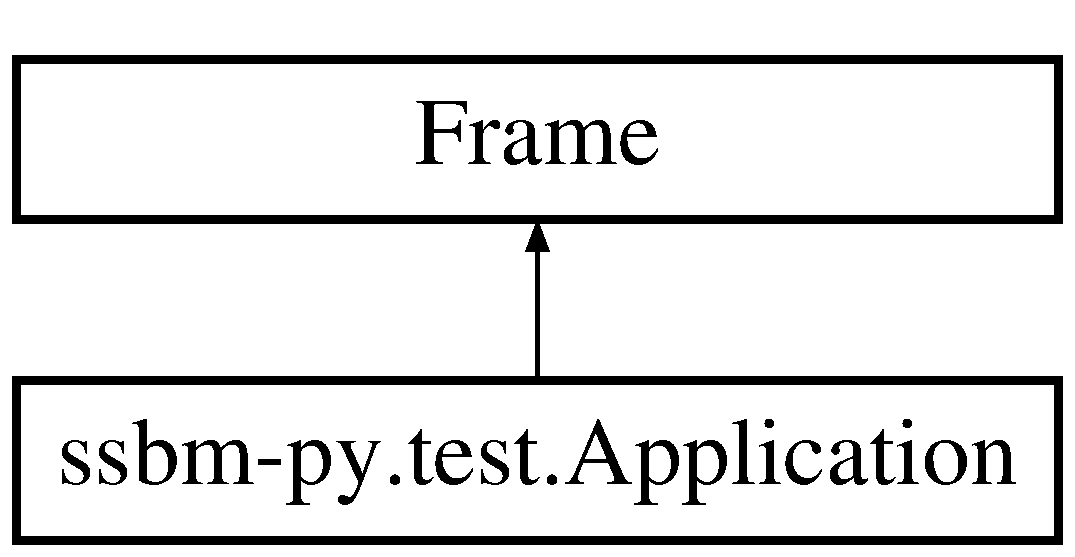
\includegraphics[height=2.000000cm]{classssbm-py_1_1test_1_1_application}
\end{center}
\end{figure}
\subsection*{Public Member Functions}
\begin{DoxyCompactItemize}
\item 
\mbox{\Hypertarget{classssbm-py_1_1test_1_1_application_a4cd1acf78c488cd4c7b35323f089fa74}\label{classssbm-py_1_1test_1_1_application_a4cd1acf78c488cd4c7b35323f089fa74}} 
def {\bfseries \+\_\+\+\_\+init\+\_\+\+\_\+} (self, master=None)
\item 
\mbox{\Hypertarget{classssbm-py_1_1test_1_1_application_ad8d1cb4e9e95923fae411c2db34e5a5f}\label{classssbm-py_1_1test_1_1_application_ad8d1cb4e9e95923fae411c2db34e5a5f}} 
def {\bfseries create\+\_\+widgets} (self)
\item 
\mbox{\Hypertarget{classssbm-py_1_1test_1_1_application_acda31132b755d4d924f77fb94abf936c}\label{classssbm-py_1_1test_1_1_application_acda31132b755d4d924f77fb94abf936c}} 
def {\bfseries say\+\_\+hi} (self)
\end{DoxyCompactItemize}
\subsection*{Public Attributes}
\begin{DoxyCompactItemize}
\item 
\mbox{\Hypertarget{classssbm-py_1_1test_1_1_application_a61b42a08e6b1e1013cafbb108a72157a}\label{classssbm-py_1_1test_1_1_application_a61b42a08e6b1e1013cafbb108a72157a}} 
{\bfseries hi\+\_\+there}
\item 
\mbox{\Hypertarget{classssbm-py_1_1test_1_1_application_a7ee8f905edc946e603586c694c641136}\label{classssbm-py_1_1test_1_1_application_a7ee8f905edc946e603586c694c641136}} 
{\bfseries quit}
\end{DoxyCompactItemize}


The documentation for this class was generated from the following file\+:\begin{DoxyCompactItemize}
\item 
test.\+py\end{DoxyCompactItemize}

\hypertarget{classssbm-py_1_1match_1_1_match}{}\section{ssbm-\/py.match.\+Match Class Reference}
\label{classssbm-py_1_1match_1_1_match}\index{ssbm-\/py.\+match.\+Match@{ssbm-\/py.\+match.\+Match}}
\subsection*{Public Member Functions}
\begin{DoxyCompactItemize}
\item 
\mbox{\Hypertarget{classssbm-py_1_1match_1_1_match_af9976cfb563fc57b35f8fdde1485daa7}\label{classssbm-py_1_1match_1_1_match_af9976cfb563fc57b35f8fdde1485daa7}} 
def {\bfseries \+\_\+\+\_\+init\+\_\+\+\_\+} (self)
\item 
def \hyperlink{classssbm-py_1_1match_1_1_match_a437a1c291dc23588076add106dcb787b}{is\+\_\+singles} (self)
\item 
def \hyperlink{classssbm-py_1_1match_1_1_match_abc1ed5b3ce5ad859ce6f0efe4c53b0c4}{get\+\_\+best\+\_\+of} (self)
\item 
def \hyperlink{classssbm-py_1_1match_1_1_match_acfdd80d2f04e2d98050447d905ab368d}{get\+\_\+set\+\_\+round} (self, round\+\_\+string)
\end{DoxyCompactItemize}
\subsection*{Public Attributes}
\begin{DoxyCompactItemize}
\item 
\mbox{\Hypertarget{classssbm-py_1_1match_1_1_match_a76110998a7c75fd7133f85b74493dcdc}\label{classssbm-py_1_1match_1_1_match_a76110998a7c75fd7133f85b74493dcdc}} 
{\bfseries player1}
\item 
\mbox{\Hypertarget{classssbm-py_1_1match_1_1_match_a77267977bea1a5aa2138040df876ad2e}\label{classssbm-py_1_1match_1_1_match_a77267977bea1a5aa2138040df876ad2e}} 
{\bfseries player2}
\item 
\mbox{\Hypertarget{classssbm-py_1_1match_1_1_match_a90b2153f1fe1138fa6727a21ef3bb22d}\label{classssbm-py_1_1match_1_1_match_a90b2153f1fe1138fa6727a21ef3bb22d}} 
{\bfseries player3}
\item 
\mbox{\Hypertarget{classssbm-py_1_1match_1_1_match_a8f045691af37d9b52eeaf2b314de60f0}\label{classssbm-py_1_1match_1_1_match_a8f045691af37d9b52eeaf2b314de60f0}} 
{\bfseries player4}
\end{DoxyCompactItemize}


\subsection{Detailed Description}
\begin{DoxyVerb}The Match class is designed to be a basic class that
holds essential information about a set. And can be modified
it contains information on the players in the match
in the form of four Player objects, labeled 1-4
note that regardless of the notation in the code,
any player can be assigned to any port. Players are accessed
by their respective accessor functions.
\end{DoxyVerb}
 

\subsection{Member Function Documentation}
\mbox{\Hypertarget{classssbm-py_1_1match_1_1_match_abc1ed5b3ce5ad859ce6f0efe4c53b0c4}\label{classssbm-py_1_1match_1_1_match_abc1ed5b3ce5ad859ce6f0efe4c53b0c4}} 
\index{ssbm-\/py\+::match\+::\+Match@{ssbm-\/py\+::match\+::\+Match}!get\+\_\+best\+\_\+of@{get\+\_\+best\+\_\+of}}
\index{get\+\_\+best\+\_\+of@{get\+\_\+best\+\_\+of}!ssbm-\/py\+::match\+::\+Match@{ssbm-\/py\+::match\+::\+Match}}
\subsubsection{\texorpdfstring{get\+\_\+best\+\_\+of()}{get\_best\_of()}}
{\footnotesize\ttfamily def ssbm-\/py.\+match.\+Match.\+get\+\_\+best\+\_\+of (\begin{DoxyParamCaption}\item[{}]{self }\end{DoxyParamCaption})}

\begin{DoxyVerb}Return the total number of games (e.g., Bo3 == 3)\end{DoxyVerb}
 \mbox{\Hypertarget{classssbm-py_1_1match_1_1_match_acfdd80d2f04e2d98050447d905ab368d}\label{classssbm-py_1_1match_1_1_match_acfdd80d2f04e2d98050447d905ab368d}} 
\index{ssbm-\/py\+::match\+::\+Match@{ssbm-\/py\+::match\+::\+Match}!get\+\_\+set\+\_\+round@{get\+\_\+set\+\_\+round}}
\index{get\+\_\+set\+\_\+round@{get\+\_\+set\+\_\+round}!ssbm-\/py\+::match\+::\+Match@{ssbm-\/py\+::match\+::\+Match}}
\subsubsection{\texorpdfstring{get\+\_\+set\+\_\+round()}{get\_set\_round()}}
{\footnotesize\ttfamily def ssbm-\/py.\+match.\+Match.\+get\+\_\+set\+\_\+round (\begin{DoxyParamCaption}\item[{}]{self,  }\item[{}]{round\+\_\+string }\end{DoxyParamCaption})}

\begin{DoxyVerb}Returns a string\end{DoxyVerb}
 \mbox{\Hypertarget{classssbm-py_1_1match_1_1_match_a437a1c291dc23588076add106dcb787b}\label{classssbm-py_1_1match_1_1_match_a437a1c291dc23588076add106dcb787b}} 
\index{ssbm-\/py\+::match\+::\+Match@{ssbm-\/py\+::match\+::\+Match}!is\+\_\+singles@{is\+\_\+singles}}
\index{is\+\_\+singles@{is\+\_\+singles}!ssbm-\/py\+::match\+::\+Match@{ssbm-\/py\+::match\+::\+Match}}
\subsubsection{\texorpdfstring{is\+\_\+singles()}{is\_singles()}}
{\footnotesize\ttfamily def ssbm-\/py.\+match.\+Match.\+is\+\_\+singles (\begin{DoxyParamCaption}\item[{}]{self }\end{DoxyParamCaption})}

\begin{DoxyVerb}Returns True if the match is a singles match \end{DoxyVerb}
 

The documentation for this class was generated from the following file\+:\begin{DoxyCompactItemize}
\item 
\hyperlink{match_8py}{match.\+py}\end{DoxyCompactItemize}

\hypertarget{classssbm-py_1_1player_1_1_player}{}\section{ssbm-\/py.player.\+Player Class Reference}
\label{classssbm-py_1_1player_1_1_player}\index{ssbm-\/py.\+player.\+Player@{ssbm-\/py.\+player.\+Player}}
\subsection*{Public Member Functions}
\begin{DoxyCompactItemize}
\item 
\mbox{\Hypertarget{classssbm-py_1_1player_1_1_player_aeb22f9b0e07e0dd274950ff502183570}\label{classssbm-py_1_1player_1_1_player_aeb22f9b0e07e0dd274950ff502183570}} 
def {\bfseries \+\_\+\+\_\+init\+\_\+\+\_\+} (self)
\item 
def \hyperlink{classssbm-py_1_1player_1_1_player_ab108135e28b39fd47eb28b698d8e7dca}{set\+\_\+tag} (self, new\+\_\+tag)
\item 
def \hyperlink{classssbm-py_1_1player_1_1_player_a25b5683581a1137b24933f56ceb5a1e5}{set\+\_\+port} (self, new\+\_\+port)
\item 
def \hyperlink{classssbm-py_1_1player_1_1_player_a48cacf185c1cb9741d9b5bbd808df68c}{set\+\_\+prefox} (self, new\+\_\+prefix)
\item 
def \hyperlink{classssbm-py_1_1player_1_1_player_ae43cdb84af3cf17196da1d9f6cda1bbd}{set\+\_\+char} (self, new\+\_\+char)
\item 
def \hyperlink{classssbm-py_1_1player_1_1_player_a6489819d117a20bc66da65479679e931}{set\+\_\+sub\+\_\+color} (self, new\+\_\+sub\+\_\+color)
\item 
def \hyperlink{classssbm-py_1_1player_1_1_player_a76ee5811187bdd2bf707aefa7fe8289f}{set\+\_\+team} (self, new\+\_\+team)
\item 
def \hyperlink{classssbm-py_1_1player_1_1_player_a249df262cf377aa1a4ad4c1a28ed4c3c}{get\+\_\+tag} (self)
\item 
def \hyperlink{classssbm-py_1_1player_1_1_player_a5773bdb0017fdbf0f329f1186d6fc9d6}{get\+\_\+port} (self)
\item 
def \hyperlink{classssbm-py_1_1player_1_1_player_a34d3df779ec8c498c71a88f08a2e3d7d}{get\+\_\+prefix} (self)
\item 
def \hyperlink{classssbm-py_1_1player_1_1_player_a9642f6dbf8c2fbe2fcabdced55fe6913}{get\+\_\+char} (self)
\item 
def \hyperlink{classssbm-py_1_1player_1_1_player_ad0147eb4ccff73c6708a23a2f6a02be4}{get\+\_\+sub\+\_\+color} (self)
\item 
def \hyperlink{classssbm-py_1_1player_1_1_player_ac9d3031930eb64515b9e836eb785237a}{get\+\_\+team} (self)
\end{DoxyCompactItemize}


\subsection{Detailed Description}
\begin{DoxyVerb}A class describing a specific player.
Used by Match, Tournament, and possible future
stat-keeping applications
\end{DoxyVerb}
 

\subsection{Member Function Documentation}
\mbox{\Hypertarget{classssbm-py_1_1player_1_1_player_a9642f6dbf8c2fbe2fcabdced55fe6913}\label{classssbm-py_1_1player_1_1_player_a9642f6dbf8c2fbe2fcabdced55fe6913}} 
\index{ssbm-\/py\+::player\+::\+Player@{ssbm-\/py\+::player\+::\+Player}!get\+\_\+char@{get\+\_\+char}}
\index{get\+\_\+char@{get\+\_\+char}!ssbm-\/py\+::player\+::\+Player@{ssbm-\/py\+::player\+::\+Player}}
\subsubsection{\texorpdfstring{get\+\_\+char()}{get\_char()}}
{\footnotesize\ttfamily def ssbm-\/py.\+player.\+Player.\+get\+\_\+char (\begin{DoxyParamCaption}\item[{}]{self }\end{DoxyParamCaption})}

\begin{DoxyVerb}An accessor for __char \end{DoxyVerb}
 \mbox{\Hypertarget{classssbm-py_1_1player_1_1_player_a5773bdb0017fdbf0f329f1186d6fc9d6}\label{classssbm-py_1_1player_1_1_player_a5773bdb0017fdbf0f329f1186d6fc9d6}} 
\index{ssbm-\/py\+::player\+::\+Player@{ssbm-\/py\+::player\+::\+Player}!get\+\_\+port@{get\+\_\+port}}
\index{get\+\_\+port@{get\+\_\+port}!ssbm-\/py\+::player\+::\+Player@{ssbm-\/py\+::player\+::\+Player}}
\subsubsection{\texorpdfstring{get\+\_\+port()}{get\_port()}}
{\footnotesize\ttfamily def ssbm-\/py.\+player.\+Player.\+get\+\_\+port (\begin{DoxyParamCaption}\item[{}]{self }\end{DoxyParamCaption})}

\begin{DoxyVerb}An accessor for __port \end{DoxyVerb}
 \mbox{\Hypertarget{classssbm-py_1_1player_1_1_player_a34d3df779ec8c498c71a88f08a2e3d7d}\label{classssbm-py_1_1player_1_1_player_a34d3df779ec8c498c71a88f08a2e3d7d}} 
\index{ssbm-\/py\+::player\+::\+Player@{ssbm-\/py\+::player\+::\+Player}!get\+\_\+prefix@{get\+\_\+prefix}}
\index{get\+\_\+prefix@{get\+\_\+prefix}!ssbm-\/py\+::player\+::\+Player@{ssbm-\/py\+::player\+::\+Player}}
\subsubsection{\texorpdfstring{get\+\_\+prefix()}{get\_prefix()}}
{\footnotesize\ttfamily def ssbm-\/py.\+player.\+Player.\+get\+\_\+prefix (\begin{DoxyParamCaption}\item[{}]{self }\end{DoxyParamCaption})}

\begin{DoxyVerb}An accessor for __prefix \end{DoxyVerb}
 \mbox{\Hypertarget{classssbm-py_1_1player_1_1_player_ad0147eb4ccff73c6708a23a2f6a02be4}\label{classssbm-py_1_1player_1_1_player_ad0147eb4ccff73c6708a23a2f6a02be4}} 
\index{ssbm-\/py\+::player\+::\+Player@{ssbm-\/py\+::player\+::\+Player}!get\+\_\+sub\+\_\+color@{get\+\_\+sub\+\_\+color}}
\index{get\+\_\+sub\+\_\+color@{get\+\_\+sub\+\_\+color}!ssbm-\/py\+::player\+::\+Player@{ssbm-\/py\+::player\+::\+Player}}
\subsubsection{\texorpdfstring{get\+\_\+sub\+\_\+color()}{get\_sub\_color()}}
{\footnotesize\ttfamily def ssbm-\/py.\+player.\+Player.\+get\+\_\+sub\+\_\+color (\begin{DoxyParamCaption}\item[{}]{self }\end{DoxyParamCaption})}

\begin{DoxyVerb}An accessor for __sub_color \end{DoxyVerb}
 \mbox{\Hypertarget{classssbm-py_1_1player_1_1_player_a249df262cf377aa1a4ad4c1a28ed4c3c}\label{classssbm-py_1_1player_1_1_player_a249df262cf377aa1a4ad4c1a28ed4c3c}} 
\index{ssbm-\/py\+::player\+::\+Player@{ssbm-\/py\+::player\+::\+Player}!get\+\_\+tag@{get\+\_\+tag}}
\index{get\+\_\+tag@{get\+\_\+tag}!ssbm-\/py\+::player\+::\+Player@{ssbm-\/py\+::player\+::\+Player}}
\subsubsection{\texorpdfstring{get\+\_\+tag()}{get\_tag()}}
{\footnotesize\ttfamily def ssbm-\/py.\+player.\+Player.\+get\+\_\+tag (\begin{DoxyParamCaption}\item[{}]{self }\end{DoxyParamCaption})}

\begin{DoxyVerb}An accessor for __tag \end{DoxyVerb}
 \mbox{\Hypertarget{classssbm-py_1_1player_1_1_player_ac9d3031930eb64515b9e836eb785237a}\label{classssbm-py_1_1player_1_1_player_ac9d3031930eb64515b9e836eb785237a}} 
\index{ssbm-\/py\+::player\+::\+Player@{ssbm-\/py\+::player\+::\+Player}!get\+\_\+team@{get\+\_\+team}}
\index{get\+\_\+team@{get\+\_\+team}!ssbm-\/py\+::player\+::\+Player@{ssbm-\/py\+::player\+::\+Player}}
\subsubsection{\texorpdfstring{get\+\_\+team()}{get\_team()}}
{\footnotesize\ttfamily def ssbm-\/py.\+player.\+Player.\+get\+\_\+team (\begin{DoxyParamCaption}\item[{}]{self }\end{DoxyParamCaption})}

\begin{DoxyVerb}An accessor for __team \end{DoxyVerb}
 \mbox{\Hypertarget{classssbm-py_1_1player_1_1_player_ae43cdb84af3cf17196da1d9f6cda1bbd}\label{classssbm-py_1_1player_1_1_player_ae43cdb84af3cf17196da1d9f6cda1bbd}} 
\index{ssbm-\/py\+::player\+::\+Player@{ssbm-\/py\+::player\+::\+Player}!set\+\_\+char@{set\+\_\+char}}
\index{set\+\_\+char@{set\+\_\+char}!ssbm-\/py\+::player\+::\+Player@{ssbm-\/py\+::player\+::\+Player}}
\subsubsection{\texorpdfstring{set\+\_\+char()}{set\_char()}}
{\footnotesize\ttfamily def ssbm-\/py.\+player.\+Player.\+set\+\_\+char (\begin{DoxyParamCaption}\item[{}]{self,  }\item[{}]{new\+\_\+char }\end{DoxyParamCaption})}

\begin{DoxyVerb}A mutator for __char \end{DoxyVerb}
 \mbox{\Hypertarget{classssbm-py_1_1player_1_1_player_a25b5683581a1137b24933f56ceb5a1e5}\label{classssbm-py_1_1player_1_1_player_a25b5683581a1137b24933f56ceb5a1e5}} 
\index{ssbm-\/py\+::player\+::\+Player@{ssbm-\/py\+::player\+::\+Player}!set\+\_\+port@{set\+\_\+port}}
\index{set\+\_\+port@{set\+\_\+port}!ssbm-\/py\+::player\+::\+Player@{ssbm-\/py\+::player\+::\+Player}}
\subsubsection{\texorpdfstring{set\+\_\+port()}{set\_port()}}
{\footnotesize\ttfamily def ssbm-\/py.\+player.\+Player.\+set\+\_\+port (\begin{DoxyParamCaption}\item[{}]{self,  }\item[{}]{new\+\_\+port }\end{DoxyParamCaption})}

\begin{DoxyVerb}A mutator for __port \end{DoxyVerb}
 \mbox{\Hypertarget{classssbm-py_1_1player_1_1_player_a48cacf185c1cb9741d9b5bbd808df68c}\label{classssbm-py_1_1player_1_1_player_a48cacf185c1cb9741d9b5bbd808df68c}} 
\index{ssbm-\/py\+::player\+::\+Player@{ssbm-\/py\+::player\+::\+Player}!set\+\_\+prefox@{set\+\_\+prefox}}
\index{set\+\_\+prefox@{set\+\_\+prefox}!ssbm-\/py\+::player\+::\+Player@{ssbm-\/py\+::player\+::\+Player}}
\subsubsection{\texorpdfstring{set\+\_\+prefox()}{set\_prefox()}}
{\footnotesize\ttfamily def ssbm-\/py.\+player.\+Player.\+set\+\_\+prefox (\begin{DoxyParamCaption}\item[{}]{self,  }\item[{}]{new\+\_\+prefix }\end{DoxyParamCaption})}

\begin{DoxyVerb}A mutator for __prefix \end{DoxyVerb}
 \mbox{\Hypertarget{classssbm-py_1_1player_1_1_player_a6489819d117a20bc66da65479679e931}\label{classssbm-py_1_1player_1_1_player_a6489819d117a20bc66da65479679e931}} 
\index{ssbm-\/py\+::player\+::\+Player@{ssbm-\/py\+::player\+::\+Player}!set\+\_\+sub\+\_\+color@{set\+\_\+sub\+\_\+color}}
\index{set\+\_\+sub\+\_\+color@{set\+\_\+sub\+\_\+color}!ssbm-\/py\+::player\+::\+Player@{ssbm-\/py\+::player\+::\+Player}}
\subsubsection{\texorpdfstring{set\+\_\+sub\+\_\+color()}{set\_sub\_color()}}
{\footnotesize\ttfamily def ssbm-\/py.\+player.\+Player.\+set\+\_\+sub\+\_\+color (\begin{DoxyParamCaption}\item[{}]{self,  }\item[{}]{new\+\_\+sub\+\_\+color }\end{DoxyParamCaption})}

\begin{DoxyVerb}A mutator for __sub_color \end{DoxyVerb}
 \mbox{\Hypertarget{classssbm-py_1_1player_1_1_player_ab108135e28b39fd47eb28b698d8e7dca}\label{classssbm-py_1_1player_1_1_player_ab108135e28b39fd47eb28b698d8e7dca}} 
\index{ssbm-\/py\+::player\+::\+Player@{ssbm-\/py\+::player\+::\+Player}!set\+\_\+tag@{set\+\_\+tag}}
\index{set\+\_\+tag@{set\+\_\+tag}!ssbm-\/py\+::player\+::\+Player@{ssbm-\/py\+::player\+::\+Player}}
\subsubsection{\texorpdfstring{set\+\_\+tag()}{set\_tag()}}
{\footnotesize\ttfamily def ssbm-\/py.\+player.\+Player.\+set\+\_\+tag (\begin{DoxyParamCaption}\item[{}]{self,  }\item[{}]{new\+\_\+tag }\end{DoxyParamCaption})}

\begin{DoxyVerb}A mutator for __tag \end{DoxyVerb}
 \mbox{\Hypertarget{classssbm-py_1_1player_1_1_player_a76ee5811187bdd2bf707aefa7fe8289f}\label{classssbm-py_1_1player_1_1_player_a76ee5811187bdd2bf707aefa7fe8289f}} 
\index{ssbm-\/py\+::player\+::\+Player@{ssbm-\/py\+::player\+::\+Player}!set\+\_\+team@{set\+\_\+team}}
\index{set\+\_\+team@{set\+\_\+team}!ssbm-\/py\+::player\+::\+Player@{ssbm-\/py\+::player\+::\+Player}}
\subsubsection{\texorpdfstring{set\+\_\+team()}{set\_team()}}
{\footnotesize\ttfamily def ssbm-\/py.\+player.\+Player.\+set\+\_\+team (\begin{DoxyParamCaption}\item[{}]{self,  }\item[{}]{new\+\_\+team }\end{DoxyParamCaption})}

\begin{DoxyVerb}A mutator for __team \end{DoxyVerb}
 

The documentation for this class was generated from the following file\+:\begin{DoxyCompactItemize}
\item 
\hyperlink{player_8py}{player.\+py}\end{DoxyCompactItemize}

\hypertarget{classssbm-py_1_1player__frames_1_1_player_frames}{}\section{ssbm-\/py.player\+\_\+frames.\+Player\+Frames Class Reference}
\label{classssbm-py_1_1player__frames_1_1_player_frames}\index{ssbm-\/py.\+player\+\_\+frames.\+Player\+Frames@{ssbm-\/py.\+player\+\_\+frames.\+Player\+Frames}}
Inheritance diagram for ssbm-\/py.player\+\_\+frames.\+Player\+Frames\+:\begin{figure}[H]
\begin{center}
\leavevmode
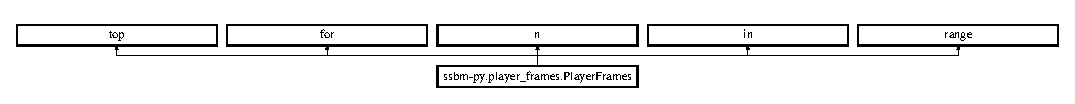
\includegraphics[height=0.945148cm]{classssbm-py_1_1player__frames_1_1_player_frames}
\end{center}
\end{figure}
\subsection*{Static Public Attributes}
\begin{DoxyCompactItemize}
\item 
\mbox{\Hypertarget{classssbm-py_1_1player__frames_1_1_player_frames_a7a2f37759856e3cce93765622b7a3b72}\label{classssbm-py_1_1player__frames_1_1_player_frames_a7a2f37759856e3cce93765622b7a3b72}} 
{\bfseries pframe} = ttk.\+Label\+Frame(f1, text = \char`\"{}Player \char`\"{} + str(n+1))
\item 
\mbox{\Hypertarget{classssbm-py_1_1player__frames_1_1_player_frames_aa7698f4badef11bc0606a7cda1c124c2}\label{classssbm-py_1_1player__frames_1_1_player_frames_aa7698f4badef11bc0606a7cda1c124c2}} 
{\bfseries column}
\item 
\mbox{\Hypertarget{classssbm-py_1_1player__frames_1_1_player_frames_ac09e048f5b118386c53ff2d8e8828abe}\label{classssbm-py_1_1player__frames_1_1_player_frames_ac09e048f5b118386c53ff2d8e8828abe}} 
{\bfseries row}
\item 
\mbox{\Hypertarget{classssbm-py_1_1player__frames_1_1_player_frames_ac8db1b1947670dcf20d114e37be97b9e}\label{classssbm-py_1_1player__frames_1_1_player_frames_ac8db1b1947670dcf20d114e37be97b9e}} 
{\bfseries tag\+\_\+label} = ttk.\+Label(player\+\_\+frames\mbox{[}n\mbox{]}, text=\char`\"{}Tag\+:\char`\"{})
\item 
\mbox{\Hypertarget{classssbm-py_1_1player__frames_1_1_player_frames_a8b8980e25b1b9144a291383bb08580a6}\label{classssbm-py_1_1player__frames_1_1_player_frames_a8b8980e25b1b9144a291383bb08580a6}} 
{\bfseries sticky}
\item 
\mbox{\Hypertarget{classssbm-py_1_1player__frames_1_1_player_frames_a688e7fe72b1c20c559befb48ade737ca}\label{classssbm-py_1_1player__frames_1_1_player_frames_a688e7fe72b1c20c559befb48ade737ca}} 
{\bfseries port\+\_\+label} = ttk.\+Label(player\+\_\+frames\mbox{[}n\mbox{]}, text=\char`\"{}Port\+:\char`\"{})
\item 
\mbox{\Hypertarget{classssbm-py_1_1player__frames_1_1_player_frames_a77dc90afb6763d2bc15f552a5a4849c6}\label{classssbm-py_1_1player__frames_1_1_player_frames_a77dc90afb6763d2bc15f552a5a4849c6}} 
{\bfseries prefix\+\_\+label} = ttk.\+Label(player\+\_\+frames\mbox{[}n\mbox{]}, text=\char`\"{}Prefix\+:\char`\"{})
\item 
\mbox{\Hypertarget{classssbm-py_1_1player__frames_1_1_player_frames_a2e25cc369bcde0cdd551bd752ba909ad}\label{classssbm-py_1_1player__frames_1_1_player_frames_a2e25cc369bcde0cdd551bd752ba909ad}} 
{\bfseries columnspan}
\item 
\mbox{\Hypertarget{classssbm-py_1_1player__frames_1_1_player_frames_a55745700c32ebdfa28c2153fbee84576}\label{classssbm-py_1_1player__frames_1_1_player_frames_a55745700c32ebdfa28c2153fbee84576}} 
{\bfseries tag} = ttk.\+Entry(player\+\_\+frames\mbox{[}n\mbox{]})
\item 
\mbox{\Hypertarget{classssbm-py_1_1player__frames_1_1_player_frames_ae82bee56c117e40554206d46e28e5905}\label{classssbm-py_1_1player__frames_1_1_player_frames_ae82bee56c117e40554206d46e28e5905}} 
{\bfseries prefix} = ttk.\+Entry(player\+\_\+frames\mbox{[}n\mbox{]})
\item 
\mbox{\Hypertarget{classssbm-py_1_1player__frames_1_1_player_frames_af0bb7f8c566f5ebf235e27d5444bfd28}\label{classssbm-py_1_1player__frames_1_1_player_frames_af0bb7f8c566f5ebf235e27d5444bfd28}} 
{\bfseries port\+\_\+dropdown} = ttk.\+Option\+Menu(player\+\_\+frames\mbox{[}n\mbox{]}, port\mbox{[}n\mbox{]}, command = lambda \+\_\+\+: update\+\_\+character(current\+\_\+match, n), $\ast$ports)
\item 
\mbox{\Hypertarget{classssbm-py_1_1player__frames_1_1_player_frames_a730c424f3370543df79e54e8355151b5}\label{classssbm-py_1_1player__frames_1_1_player_frames_a730c424f3370543df79e54e8355151b5}} 
{\bfseries char\+\_\+dropdown} = ttk.\+Option\+Menu(player\+\_\+frames\mbox{[}n\mbox{]}, char\mbox{[}n\mbox{]}, command = lambda \+\_\+\+: update\+\_\+character(current\+\_\+match, n), $\ast$character\+\_\+names)
\item 
\mbox{\Hypertarget{classssbm-py_1_1player__frames_1_1_player_frames_a9209cb184ae4224d6e03f0acb9f35261}\label{classssbm-py_1_1player__frames_1_1_player_frames_a9209cb184ae4224d6e03f0acb9f35261}} 
{\bfseries char\+\_\+prevcolor} = ttk.\+Button(player\+\_\+frames\mbox{[}n\mbox{]}, text = \char`\"{}$<$\char`\"{}, width=1)
\item 
\mbox{\Hypertarget{classssbm-py_1_1player__frames_1_1_player_frames_a699f4496eb8ad385d0a104f6cd0c1e22}\label{classssbm-py_1_1player__frames_1_1_player_frames_a699f4496eb8ad385d0a104f6cd0c1e22}} 
{\bfseries command}
\item 
\mbox{\Hypertarget{classssbm-py_1_1player__frames_1_1_player_frames_a11ca7c41610b00eed41f755113cd0346}\label{classssbm-py_1_1player__frames_1_1_player_frames_a11ca7c41610b00eed41f755113cd0346}} 
{\bfseries i}
\item 
\mbox{\Hypertarget{classssbm-py_1_1player__frames_1_1_player_frames_a1cb7ad20a5141b76cc3193a6e39c39e4}\label{classssbm-py_1_1player__frames_1_1_player_frames_a1cb7ad20a5141b76cc3193a6e39c39e4}} 
{\bfseries char\+\_\+icon} = ttk.\+Label(player\+\_\+frames\mbox{[}n\mbox{]}, image = tkimgs\mbox{[}n\mbox{]})
\item 
\mbox{\Hypertarget{classssbm-py_1_1player__frames_1_1_player_frames_a3b26f77f00b994f44fa81551f9b215ad}\label{classssbm-py_1_1player__frames_1_1_player_frames_a3b26f77f00b994f44fa81551f9b215ad}} 
{\bfseries char\+\_\+nextcolor} = ttk.\+Button(player\+\_\+frames\mbox{[}n\mbox{]}, text = \char`\"{}$>$\char`\"{}, width=1)
\end{DoxyCompactItemize}


The documentation for this class was generated from the following file\+:\begin{DoxyCompactItemize}
\item 
player\+\_\+frames.\+py\end{DoxyCompactItemize}

\chapter{File Documentation}
\hypertarget{challonge__import_8py}{}\section{challonge\+\_\+import.\+py File Reference}
\label{challonge__import_8py}\index{challonge\+\_\+import.\+py@{challonge\+\_\+import.\+py}}

\hypertarget{file__manip_8py}{}\section{file\+\_\+manip.\+py File Reference}
\label{file__manip_8py}\index{file\+\_\+manip.\+py@{file\+\_\+manip.\+py}}
\subsection*{Functions}
\begin{DoxyCompactItemize}
\item 
\mbox{\Hypertarget{file__manip_8py_a6a8768d194cd326b8aab27f728e9b08a}\label{file__manip_8py_a6a8768d194cd326b8aab27f728e9b08a}} 
def {\bfseries ssbm-\/py.\+file\+\_\+manip.\+gen\+\_\+char\+\_\+filename} (match, player)
\item 
\mbox{\Hypertarget{file__manip_8py_a216829332e8d1959bce36fc84eadd8ae}\label{file__manip_8py_a216829332e8d1959bce36fc84eadd8ae}} 
def {\bfseries ssbm-\/py.\+file\+\_\+manip.\+write\+\_\+stock\+\_\+icons} (match)
\item 
\mbox{\Hypertarget{file__manip_8py_aa35563074e065921f1485b83c4dd0a29}\label{file__manip_8py_aa35563074e065921f1485b83c4dd0a29}} 
def {\bfseries ssbm-\/py.\+file\+\_\+manip.\+write\+\_\+team\+\_\+names} ()
\end{DoxyCompactItemize}


\subsection{Detailed Description}
\begin{DoxyAuthor}{Author}
Jeff Podolski 
\end{DoxyAuthor}

\hypertarget{information_8py}{}\section{information.\+py File Reference}
\label{information_8py}\index{information.\+py@{information.\+py}}
\subsection*{Variables}
\begin{DoxyCompactItemize}
\item 
list {\bfseries ssbm-\/py.\+information.\+character\+\_\+names}
\end{DoxyCompactItemize}


\subsection{Detailed Description}
\begin{DoxyAuthor}{Author}
Jeff Podolski 
\end{DoxyAuthor}


\subsection{Variable Documentation}
\mbox{\Hypertarget{information_8py_file_a49cd688cee7adec363594c8875a6b911}\label{information_8py_file_a49cd688cee7adec363594c8875a6b911}} 
\index{information.\+py@{information.\+py}!character\+\_\+names@{character\+\_\+names}}
\index{character\+\_\+names@{character\+\_\+names}!information.\+py@{information.\+py}}
\subsubsection{\texorpdfstring{character\+\_\+names}{character\_names}}
{\footnotesize\ttfamily list ssbm-\/py.\+information.\+character\+\_\+names}

{\bfseries Initial value\+:}
\begin{DoxyCode}
1 =  [
2     \textcolor{stringliteral}{"Fox"},
3     \textcolor{stringliteral}{"Falco"},
4     \textcolor{stringliteral}{"Marth"},
5     \textcolor{stringliteral}{"Sheik"},
6     \textcolor{stringliteral}{"Jigglypuff"},
7     \textcolor{stringliteral}{"Peach"},
8     \textcolor{stringliteral}{"Captain Falcon"},
9     \textcolor{stringliteral}{"Ice Climbers"},
10     \textcolor{stringliteral}{"Samus"},
11     \textcolor{stringliteral}{"Pikachu"},
12     \textcolor{stringliteral}{"Luigi"},
13     \textcolor{stringliteral}{"Yoshi"},
14     \textcolor{stringliteral}{"Doctor Mario"},
15     \textcolor{stringliteral}{"Ganondorf"},
16     \textcolor{stringliteral}{"Mario"},
17     \textcolor{stringliteral}{"Young Link"},
18     \textcolor{stringliteral}{"Link"},
19     \textcolor{stringliteral}{"Donkey Kong"},
20     \textcolor{stringliteral}{"Mr. Game & Watch"},
21     \textcolor{stringliteral}{"Roy"},
22     \textcolor{stringliteral}{"Mewtwo"},
23     \textcolor{stringliteral}{"Zelda"},
24     \textcolor{stringliteral}{"Pichu"},
25     \textcolor{stringliteral}{"Ness"},
26     \textcolor{stringliteral}{"Bowser"},
27     \textcolor{stringliteral}{"Kirby"},
28     \textcolor{stringliteral}{"Generic"}
29 ]
\end{DoxyCode}

\hypertarget{match_8py}{}\section{match.\+py File Reference}
\label{match_8py}\index{match.\+py@{match.\+py}}
\subsection*{Classes}
\begin{DoxyCompactItemize}
\item 
class \hyperlink{classssbm-py_1_1match_1_1_match}{ssbm-\/py.\+match.\+Match}
\end{DoxyCompactItemize}


\subsection{Detailed Description}
\begin{DoxyAuthor}{Author}
Jeff Podolski 
\end{DoxyAuthor}
\begin{DoxyRefDesc}{Todo}
\item[\hyperlink{todo__todo000002}{Todo}]
\begin{DoxyItemize}
\item Make these storable and serializable
\item Have a table of possible rounds (G\+F2, Pools, W\+SF, etc.)
\item Make more comprehensive (date, tournament, etc) 
\end{DoxyItemize}\end{DoxyRefDesc}

\hypertarget{player_8py}{}\section{player.\+py File Reference}
\label{player_8py}\index{player.\+py@{player.\+py}}
\subsection*{Classes}
\begin{DoxyCompactItemize}
\item 
class \hyperlink{classssbm-py_1_1player_1_1_player}{ssbm-\/py.\+player.\+Player}
\end{DoxyCompactItemize}


\subsection{Detailed Description}
\begin{DoxyAuthor}{Author}
Jeff Podolski 
\end{DoxyAuthor}

%--- End generated contents ---

% Index
\backmatter
\newpage
\phantomsection
\clearemptydoublepage
\addcontentsline{toc}{chapter}{Index}
\printindex

\end{document}
